\documentclass[12pt]{article}

\usepackage[utf8]{inputenc}
\usepackage[polish]{babel}
\usepackage[T1]{fontenc}
\usepackage{indentfirst}
\usepackage{polski}
\usepackage{graphicx} 
\usepackage{float}
\usepackage{color}   %May be necessary if you want to color links
\usepackage{hyperref}

\hypersetup{
    colorlinks=true, %set true if you want colored links
    linktoc=all,     %set to all if you want both sections and subsections linked
    linkcolor=black,  %choose some color if you want links to stand out
}




\usepackage[top=2cm, bottom=2cm, left=3cm, right=3cm]{geometry}
\makeatletter
\newcommand{\linia}{\rule{\linewidth}{0.4mm}}
\renewcommand{\maketitle}{\begin{titlepage}
		\vspace*{1cm}
		\begin{center}\small
			Poliechnika Śląska\\
			Wydział Automatyki, Elektroniki i Informatyki\\
			Raport końcowy z Systemów Mikroprocesorowych
		\end{center}
		\vspace{3cm}
		\noindent\linia
		\begin{center}
			\LARGE \textsc{\@title}
		\end{center}
		\linia
		\vspace{0.5cm}
		\begin{flushright}
			\begin{minipage}{15cm}
				\textit{\small Autorzy:}\\
				\normalsize \textsc{Kamil Choiński} \par \textsc{Oskar Stabla} \par
			\end{minipage}	
		\end{flushright}
		\vspace*{\stretch{6}}
		\begin{center}
			\@date
		\end{center}
	\end{titlepage}
}
\makeatother

\title{Plantie™}

\begin{document}
\maketitle

\tableofcontents


\section{Ogólny opis projektu}


\subsection{Cel i zakres projektu}
Nasz projekt ma na celu pomoc zabieganym ludziom, którzy nie mają czasu na zajmowanie się
swoją ukochaną roślinką przez swój częsty brak pobytu w domu. Wystarczy dostęp do internetu,
nic więcej.

Nasza koncepcja opiera się na systemie zdalnego zarządzania rośliną. Chcemy mierzyć parametry
gleby i otoczenia takie jak wilgotność, nasłonecznienie. W zależności od odczytanych wartości przez
płytkę rozwojową UNO połączoną z modułem ESP8266 będzie możliwe sterowanie pompką wody,
lampą. Mamy zamiar połączyć projekt z IT, dlatego panel sterowania będzie umieszczony na stronie
internetowej.


\subsection{Kosztorys}
Większość komponentów projektu została sprowadzona z chin, ze względu na ich niską cenę. Niestety czas oczekiwania na nie wydłużył się i spowodował nieoczekiwane opóźnienia w harmonogramie.

\begin{table}[!h]
\centering
\begin{tabular}{l|r}
Item & Cena \\\hline
Płytka rozwojowa UNO & 10 PLN \\
Moduł ESP8266 & 18 PLN \\

Czujnik wilgotności powietrza & 5 PLN \\

Czujnik wilgotności gleby & 5 PLN \\

Czujnik nasłonecznienia & 5 PLN \\

Przetwornik & 5 PLN \\

Żarówka & 5 PLN \\

Kabelki, płytka uniwersalna, cyna, klej na gorąco & 10 PLN 
\\ \hline
Suma & 58 PLN

\end{tabular}
\caption{\label{tab:widgets}Zakupione produkty}
\end{table}

\subsection{Opis podobnych rozwiązań }
\subsubsection{Jakis z neta}
x
\subsubsection{Jakiś z neta 2}
x


\section{Szczegółowy opis projektu}


\subsection{Rozwiązania techniczne - Przegląd modułów projektu}
\subsubsection{Czujnik wilgotności i temperatury powietrza: DHT11}
 Pomiary wilgotności i temperatury powietrza są wykonywane z użyciem czujnika DHT11. Musieliśmy użyć do implementacji w ArduinoIDE biblioteki DHT-sensor-library, aby pomiary wykonywały się poprawnie.
\begin{figure}[!h]
	\begin{center}
		{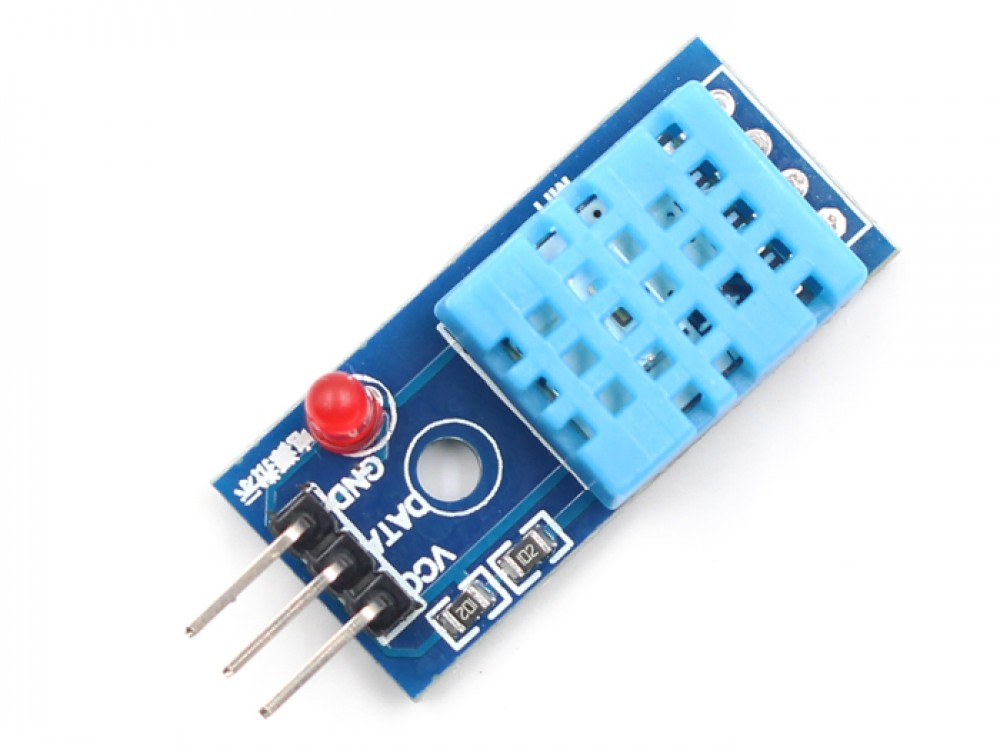
\includegraphics[width=10cm]{DHT11_photo.png}}
	\end{center}
	\caption{Czujnik DHT11}
\end{figure}

\subsubsection{Czujnik natężenia światła}
 Pomiary natężenia aktualnego oświetlenia w otoczeniu rośliny są wykonywane z użyciem czujnika natężenia światła. 
\begin{figure}[!h]
	\begin{center}
		{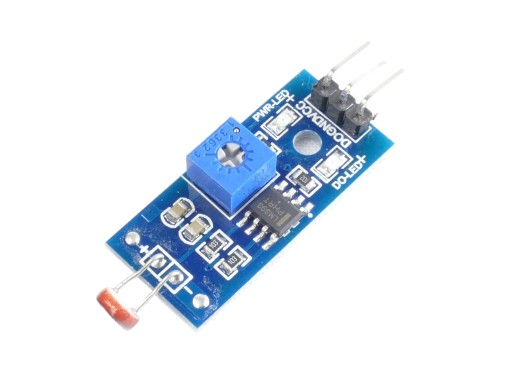
\includegraphics[width=12cm]{light_sensor_photo.png}}
	\end{center}
	\caption{Czujnik natężenia światła}
\end{figure}
\subsubsection{Czujnik wilgotności gleby FC-28}
 Pomiary aktualnej wilgotności gleby w glebie naszej rośliny są wykonywane z użyciem czujnika wilgotności gleby FC-28.

\begin{figure}[!h]
	\begin{center}
		{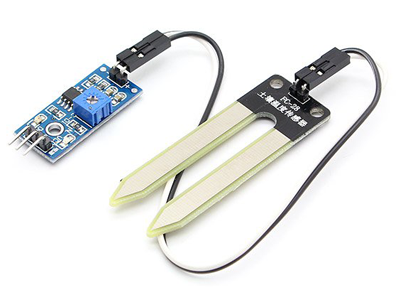
\includegraphics[width=12cm]{FC-28_photo.png}}
	\end{center}
	\caption{Czujnik FC-28}
\end{figure}
\subsubsection{Czujnik poziomu wody w zbiorniku}

\begin{figure}[!h]
	\begin{center}
		{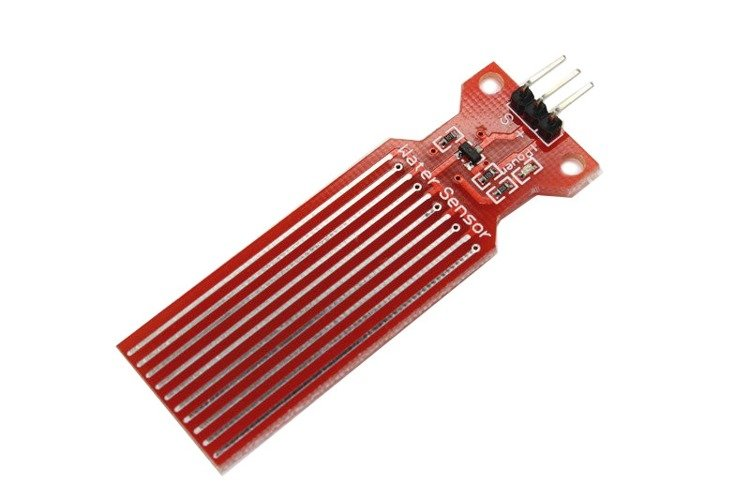
\includegraphics[width=12cm]{water_sensor_photo.png}}
	\end{center}
	\caption{Czujnik poziomu wody}
\end{figure}

\subsubsection{Wyświetlacz OLED}
Zewnętrzne wyświetlanie pomiarów wilgotności gleby i powietrza jest obsługiwane przez wyświetlacz OLED zamontowany na przodzie roślinki, aby była możliwość monitorowania jej stanu, gdy przebywamy w jej otoczeniu bez użycia połączenia internetowego. Do wypisywania danych na ekranie musieliśmy użyć bibliotek AdafruitGFX.h i  AdafruitSSD1306.h, aby poprawnie je wyświetlać. 

\begin{figure}[!h]
	\begin{center}
		{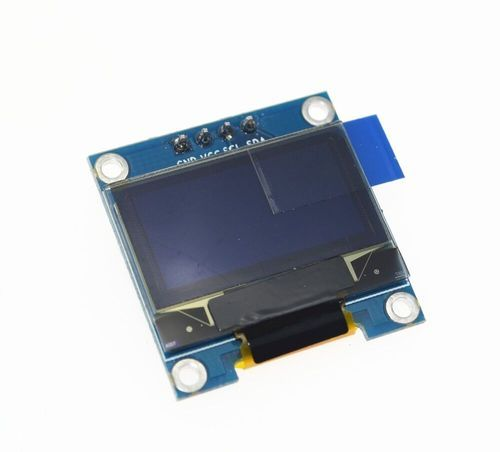
\includegraphics[width=12cm]{oled-display_photo.png}}
	\end{center}
	\caption{0.96 calowy wyświetlacz OLED}
\end{figure}
\subsubsection{Pompka wodna}


\subsubsection{Panel sterowania przez Internet: ESP8266}
Realizacja?

\subsection{Szczególne rozwiązania warstwy programowej}
\subsubsection{Płytka rozwojowa UNO}
\begin{figure}[!h]
	\begin{center}
		{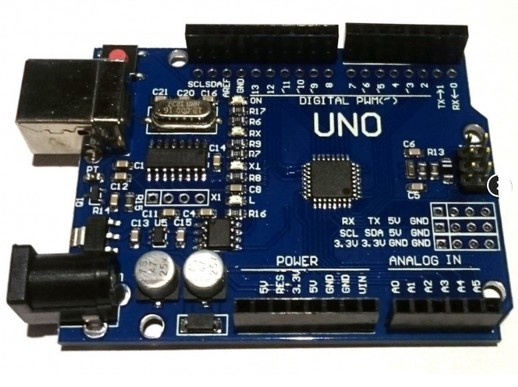
\includegraphics[width=12cm]{uno_photo.png}}
	\end{center}
	\caption{Płytka rozwojowa UNO}
\end{figure}
\subsubsection{ESP8266}
\begin{figure}[!h]
	\begin{center}
		{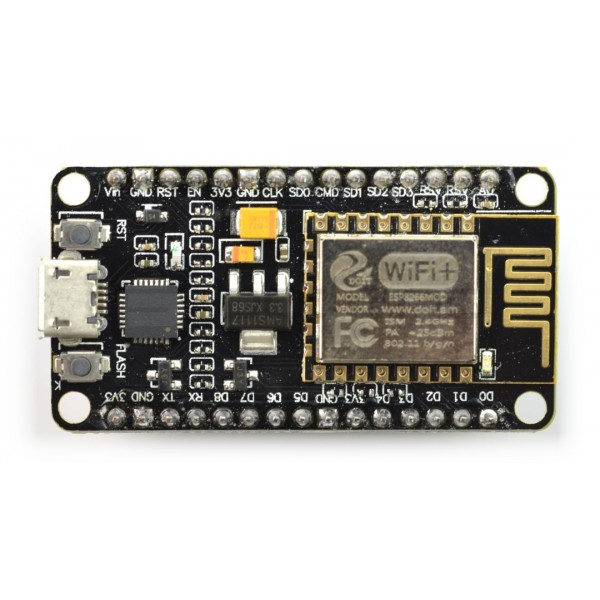
\includegraphics[width=12cm]{esp8266_photo.png}}
	\end{center}
	\caption{ESP8266}
\end{figure}
\subsubsection{Panel sterowania na serwerze}

\section{Realizacja projektu}
\subsection{Problematyka projektu}
Przed rozpoczęciem prac nad projektem .. 

\subsection{Sposób wykonania}
Postanowiliśmy połączyć płytkę rozwojową UNO obsługującą pompkę i monitorującą wartości naszych czujników z ESP8266, aby była możliwość sterowania poprzez Internet.
\subsection{Problemy napotkane podczas realizacji}
\subsubsection{Połączenie między UNO, a ESP8266}
Próbowaliśmy różnych typów połączeń jak I2C, albo SPI jednak poprawność testowych danych jakie otrzymywaliśmy była nikła - albo dostawaliśmy tylko cześć danych albo były one w różny sposób powielone.
Rozwiazaliśmy ten problem poprzez użycie wskaźników początku ''<'' i końca ''>'' przy wysyłaniu danej komendy, aby wykonać określoną czynność lub odesłać pomiary. 

\section{Postępy prac na dzień 25.11 @@@@@ do wyjebania sekcja chyba}
Podczas ostatnich tygodni skupiliśmy się na realizacji stabilnego połączenia między płytką rozwojową UNO i modułem ESP8266, a także między modułem ESP8266 i panelem sterowania na serwerze.

Zaimplementowaliśmy pomiary wilgotności i temperatury powietrza z użyciem czujnika DHT11. Musieliśmy użyć do implementacji w ArduinoIDE biblioteki DHT-sensor-library, aby pomiary wykonywały się poprawnie.

Płytka rozwojowa UNO cały czas czeka na przychodzące dane które będą zawarte w wskaźnikach początku ''<'' i końca ''>'' danej komendy, aby wykonać określoną czynność lub odesłać pomiary wykonane przez czujnik wilgotności i temperatury do ESP8266, które jest połączone z UNO poprzez piny RX i TX. UNO odsyła swoje komendy również w wskaźnikach początku i końca, aby zapobiec ''gubieniu'' danych.

ESP8266 jest naszym tzw. ''mostem'' i w każdym momencie czeka na dane czy to z UNO czy ze strony internetowej i w zależności od kogo dane otrzymuje przerzuca je do danego odbiorcy.
Program na ESP jest zrealizowany z użyciem bibliotek ESP8266WiFi, WebSocketClient, SoftwareSerial, które kolejno służą do: umożliwieniu połączenia się ESP do sieci WiFi zadeklarowanej w naszym kodzie, połączeniu się poprzez websocket jako klient do naszego serwera postawionego na laptopie, połączenia się poprzez piny RX i TX do płytki rozwojowej UNO.

Zaimplementowaliśmy testowy kod, aby pokazać postępy naszej dotychczasowej pracy. Po naciśnięciu przycisku Water na stronie przesyłana jest komenda do UNO, które zapala diodę LED. Po naciśniuęciu przycisku Fertilise gasi ją i wysyła obecne pomiary czujnika DHT11 do serwera poprzez websocket.



\section{Harmonogram i podział obowiązków}

\subsection{Podział obowiązków}

\subsection{Wstępny schemat blokowy}
Przed rozpoczęciem pracy nad projektem stworzyliśmy schemat, którego staraliśmy się trzymać jednak ze względu na pewne komplikacje w trakcie realizacji pewne aspekty zostały zmienione co zostało przedstawione na finalnym schemacie blokowym.
\begin{figure}[!h]
	\begin{center}
		{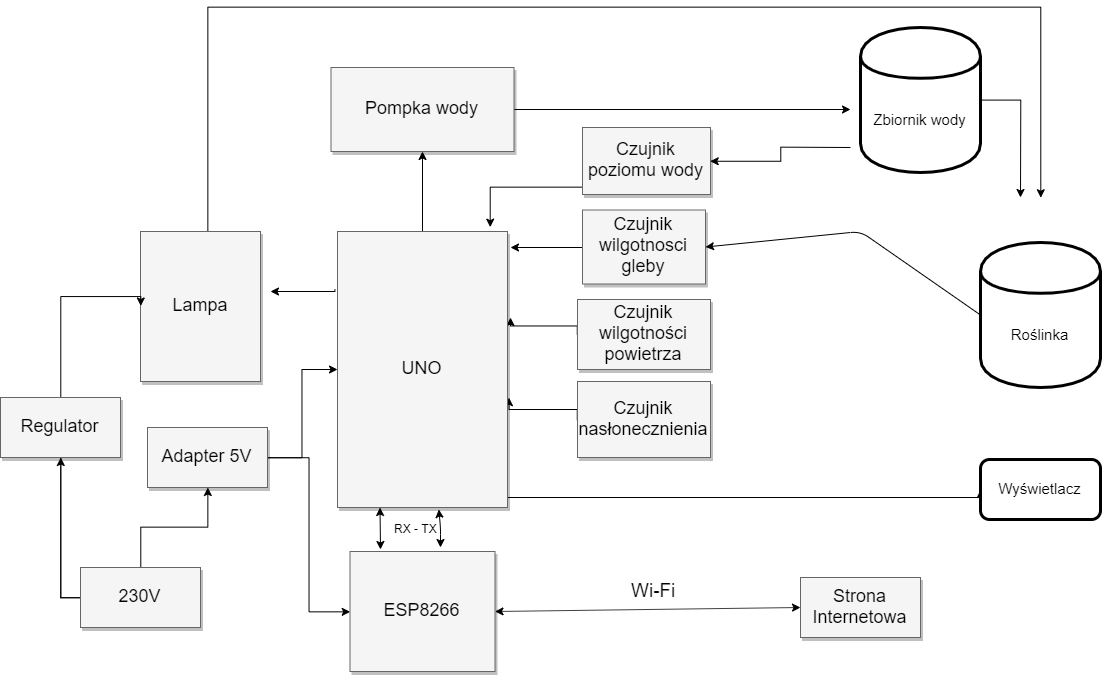
\includegraphics[width=16cm]{schemat_blokowy.png}}
	\end{center}
	\caption{Wstępny schemat blokowy}
\end{figure}


\subsection{4.11}
Przeanalizowanie schematów płytki rozwojowej UNO, modułu komunikacyjnego ESP8266, czujnika wilgotności gleby, czujnika wilgotności powietrza, czujnika nasłonecznienia oraz rozwiązanie techniczne doświetlania rośliny. Stworzenie schematu elektrycznego gotowego projektu. Testowanie poprawności działania posiadanych czujników w warunkach domowych. Implementacja komunikacji z modułem ESP8266. Dopasowywanie czasów działania. 
Dokupienie brakujących komponentów gotowego projektu. 
\subsection{25.11}
Realizacja połączeń elektrycznych na płytce stykowej i ostateczne testowanie poprawności dzia-
łania. Przeniesienie projektu na płytkę uniwersalną. Przygotowanie ewentualnej obudowy i realiza-
cja montażu systemu doświetlania. Stworzenie prezentacji na zajęcia

\subsection{16.12}
Wstępna prezentacja gotowego projektu i ocena błędów.

\subsection{20.01}
Ostateczna prezentacja z poprawką błędów.



\section{Zgodność z harmonogramem}
\subsection{4.11}
Rozpoczęliśmy prace nad naszym projektem. Postanowiliśmy skorzystać z aplikacji internetowej Trello do utworzenia tabel, które pozwoliły by nam na lepsze zarządzanie podziałem prac nad projektem.

Przeanalizowaliśmy schematy płytki rozwojowej UNO, modułu komunikacyjnego ESP8266, czujnika wilgotności gleby, czujnika wilgotności powietrza oraz czujnika nasłonecznienia. Przeanalizowaliśmy działanie każdego z czujników poprzez wykonanie przykładowych kodów na płytce rozwojowej UNO. Dowiedzieliśmy się jakich komponentów projektu nam brakuje i zamówiliśmy je w wybranych sklepach.
Stworzyliśmy wstępny schemat blokowy projektu, aby ukazać działanie poszczególnych elementów zawartych w naszym projekcie. Na ten moment postanowiliśmy nie tworzyć schematu elektrycznego, gdyż nie wiedzieliśmy jak dokładnie zrealizujemy poszczególne połączenia.

Ze względu na obszerność testowania i planowanie realizacji planu działania na nadchodzące tygodnie nie zajęliśmy się komunikacją z modułem ESP8266, ani problemem związanym z doświetlaniem naszej rośliny.


\subsection{25.11}
Do tego dnia zajmowaliśmy się komunikacją między płytką rozwojową UNO, ESP8266, a stroną internetową. Napotkaliśmy wiele problemów co nieplanowanie wydłużyło nam pracę na tym etapie projektu. Udało nam się uzyskać mniej więcej stabilne połączenie między naszymi urządzeniami. Zrealizowaliśmy połączenia UNO, ESP8266, a także podłączyliśmy do układu czujnik wilgotności i temperatury powietrza i na płytce stykowej po czym przetestowaliśmy poprawność działania. 

Przeniesienie projektu na płytkę uniwersalną okazało się niepraktyczne na tym etapie projektu, gdyż nie próbowaliśmy jeszcze połączyć ze sobą wszystkich modułów projektu i finalny kod do wgrania na UNO i ESP8266 nie był gotowy. Z powodu niewiedzy jak dokładnie będzie wyglądało nasze urządzenie na płytce uniwersalnej nie przygotowaliśmy planowanej obudowy. Nie zrealizowaliśmy również systemu doświetlania.

\subsection{16.12}
Wstępna prezentacja gotowego projektu i ocena błędów.

\subsection{20.01}
Ostateczna prezentacja z poprawką błędów.



\section{Podsumowanie }
\subsection{Pomysły na rozwój projektu }
\begin{thebibliography}{9}


\bibitem{latexcompanion} 
Michel Goossens, Frank Mittelbach, and Alexander Samarin. 
\textit{The \LaTeX\ Companion}. 
Addison-Wesley, Reading, Massachusetts, 1993.

\bibitem{latexcompanion} 
Ivan Grokhotkov
\textit{ESP8266 Arduino Core’s documentation}. 
2017

\bibitem{latexcompanion} 
Christian Klippel, Peter Andersson, Peter Lerup
\textit{ESP8266 core for Arduino}. 
2017

\bibitem{latexcompanion} 
guy
\textit{w3schools.com}. 
1999-2019
 
\bibitem{einstein} 
Albert Einstein. 
\textit{Zur Elektrodynamik bewegter K{\"o}rper}. (German) 
[\textit{On the electrodynamics of moving bodies}]. 
Annalen der Physik, 322(10):891–921, 1905.
 
\bibitem{knuthwebsite} 
Knuth: Computers and Typesetting,
\\\texttt{http://www-cs-faculty.stanford.edu/\~{}uno/abcde.html}
\end{thebibliography}


\end{document}
